\section{Demonstrator}\label{sec:demonstrator}



%\eric{My proposal: Based on Veoneer input, we give a short description of the takeover-scenario. If possible, some details about its implementation. I made sure to ask (some of) the questions in Section 5.2. From the responses, it became clear that these questions are a) relevant and b) not trivially answered based on any other system engineering artifact. Thus, we consider the SoS viewpoint (despite some need for further development) useful and important. }


%\eric{Trying to propose some content here.}
%\ins{
In this section we demonstrate the value of the SoS viewpoint described in this paper and consequently also of the architecture framework that has been proposed in~\cite{JSA2017}.
Specifically, we base the validation on our experience of applying the SoS viewpoint to a \emph{take-over} scenario.
This is an additional scenario with respect to those described in Section~\ref{sec:scenarios} and it is described here in the following.
In this scenario, three cars participate. As shown in Figure~\ref{fig:overtaking}, 
Car A is the overtaking car, Car B is the car that is overtaken, and Car C is an oncoming car that makes the overtaking maneuver risky.
Car A and Car B engage in car-to-car communication, whilst Car C is not equipped with such equipment leaving Car C silent.
As soon as the driver of Car A indicates her goal to overtake, Car B will share information of its sensors.
This will help to issue a take-over warning, even though the sensors of Car A have no way of seeing the oncoming Car C.
In this way, Car B is extending the sensor range of Car A.
%}

\begin{figure}[htb]
	\centering
	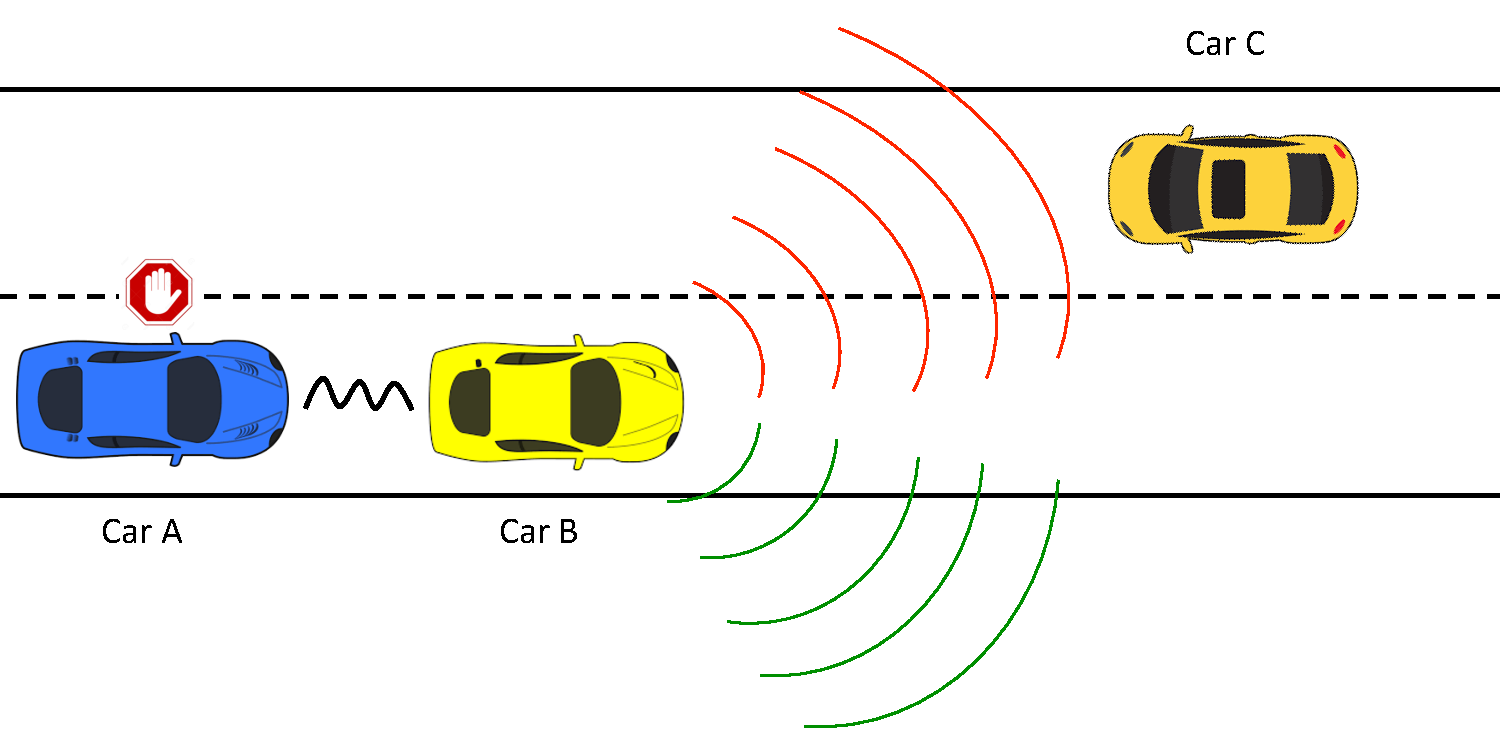
\includegraphics[width=\linewidth]{Figures/overtaking.pdf}
	\caption{Demonstrator overview}
	\label{fig:overtaking}
\end{figure}

%\ins{
This scenario has been demonstrated as part of the NGEA project, showing different triggers for indicating an imminent take-over action.
The demonstrator was based on a single Tier-1 supplier's technology stack integrated into three cars of the same brand.
While this demonstrator is a milestone towards making such technology available, it is only a first step towards engineering a system-of-systems that can effectively make overtaking safer.
%}

%\ins{
During a workshop with representatives of several participating companies, we applied the stakeholder concerns from our SoS viewpoint (see Table~\ref{tab:sos-concerns}). 
While we cannot share technical details regarding the answer to the questions, we present an argument for each to show its relevance and usefulness.
%}

\begin{longtable}{p{0.4\textwidth}p{0.55\textwidth}}
\caption{Validation of Concerns from SoS Viewpoint}\\
\small
\label{tab:sos-concerns}
%\begin{tabular}{v{0.4\textwidth}v{0.55\textwidth}}
%\toprule
\textbf{Concern} & \textbf{Validation argument}\\
%\tabularnewline
%\midrule
\hline
\endhead
Once the car is part of a SoS, how to guarantee functional safety requirements? & 
The take-over scenario clearly refers to safety-critical functions. 
Issuing a false warning, or not issuing a warning when over-taking is dangerous, could endanger the vehicles and their occupants. 
Functional safety depends on the interplay of Car A and Car B.\\
\hline
%\tabularnewline
%\hline
Once the car is part of a SoS, what are the implication on system design and functional distribution for functional safety? & 
It is clear that it is the responsibility of Car A to determine whether over-taking is safe. 
For that, there should be proper interoperability between Car A and Car B, and Car A must establish that the data received from Car B is sufficiently accurate and timely.\\
%\tabularnewline
\hline
Once functional safety requirements involve devices that are outside of the vehicle (other constituent systems of the SoS), how to ensure that these requirements will be guaranteed?
& 
This question points towards the need to enable reasoning about safety and data quality at runtime. 
Protocols and interfaces as well as reasoning about trust will become important areas.
It is in fact impossible to assess safety concerns once and for all and to relate them to the sensors and devices of a car, in this case Car A.
As we said before, Car A is extended by the devices in Car B.
In other similar scenarios Car A could be extended with devices of other cars, depending on when another instance of the taking-over scenario would happen.
This implies also that the evaluation of ``trustable" vehicle should be done by the car that want to overtake, in this case Car A, when another vehicle that is functional to the realization of the scenario is met.\\
%\tabularnewline
\hline
How the methods and processes for end-to-end function development and continuous delivery of software need to evolve to be suitable in a System of Systems setting? & 
%\eric{Bit unsure about this question}
Pushing an update or a new feature to one of the vehicles might compromise the interoperability of the vehicles.
In this sense, the delivery of new software to the car should seriously take into account not only the functionalities of the isolated vehicle but also the SoS scenarios that a vehicle is engineered for serving as a constituent of a SoS.\\
%\tabularnewline
\hline
How to enable a reliable and efficient communication between the vehicle and heterogeneous entities, like other vehicles, road signals, pedestrians, etc.?
& 
While technical feasibility has been shown in the demonstrator, it remains unclear to what extend this can be achieved with various technology stacks by different vendors.
Aspect of disturbances, adverse weather conditions, etc., should be also taken into account.\\
%\tabularnewline
\hline
How to be sure that the vehicle and other constituent systems of the SoS will be able to exchange information and to use the information that has been exchanged?
& 
While the technical feasibility of the exchange has been shown, the usage depends on advanced standards and protocols that allow for runtime reasoning.
Also, this is a good example to show that exchanging data is not enough; there is need for proper interoperability.
Referring to Section~\ref{sec:interoperability}, we need a communication protocol, and the connected vehicles need to be able to communicate.
However, they should be also able to properly understand and interpret the exchanged messages (semantic interoperability).
Moreover, the vehicles will behave assuming that the exchanged data will have the effects they expect on the other vehicle (pragmatic interoperability).
Time is also an important aspect since Car A would need timely data from Car B and data soon become obsolete (dynamic interoperability).
This scenario is not so complex from the point of view of interoperability, since it basically only requires some data sent from Car B to Car A when Car A asks for that.
In this sense, a level of conceptual interoperability is probably not necessary.\\
%\tabularnewline
\hline
How to guarantee that the security of the vehicle is preserved once the vehicle becomes connected?
& 
This question was deemed relevant during the workshop, requiring advanced protocols that allow to verify and compute trust in data.\\
%\tabularnewline
\hline
How to identify the right tradeoff between shared data and users' privacy?
&
This question points towards constraints for the solution space of the questions above, since it makes solutions favorable that do not store the id of the individual cars.\\
%\tabularnewline
\hline
How to keep the data shared within the SoS (and possible replication of data) sufficiently updated or synchronized? & 
%\ins{
This concern was considered relevant, since it requires the consideration of recording critical information. 
%}
\\
%\tabularnewline
\hline
How to manage the age of available information? & 
The take-over scenario requires current information.
As discussed above this is important for having a proper interoperability among the vehicles, specifically for having dynamic interoperability.\\
%\tabularnewline
\hline
Which functions in the car are allowed to make use of data coming from other constituents?
&
This concern was regarded crucial for designing the SoS. 
Clearly, a specialized component will be required to collect external data and to judge whether it is trustworthy and has sufficient quality for different usage within the car.\\
\hline
%\tabularnewline
%\bottomrule
%\end{tabular}
\end{longtable}
